%form: dc_form_05-07.tex ; user: dc_05-07_purpose_plan_rights.tex
%========== DC =========
%===== p. 05-07 研究の目的・内容、特色、計画、人権 =============
\subsection{研究の目的・内容}
%watermark: w02_purpose_plan_ugly_dc
\newcommand{\研究目的}{%
%begin  研究目的と内容===================
	\noindent
	●\textbf{研究目的}

	本研究では、SNS上でフェイクニュースの拡散を抑制するために、早期自動検出の精度向上と説明可能性の付与を目的とする。
	具体的には、(1)\textbf{生成されたコメントを使用した分類で精度が0.9を上回る手法の確立}と、
	(2)\textbf{生成されたコメントからユーザへ説明可能性を提案する手法の確立}を目指す研究を行う。

	\noindent
	●\textbf{研究方法・研究内容}

	\noindent
	(1) 生成されたコメントを使用した分類で精度が0.9を上回る手法の確立: 

	ユーザから信用が得られない狼少年的なモデルではなく、\textbf{的確にフェイクニュースだけを発見させることが可能なモデル}を構築する。
	また、性能向上に向く大規模データセットがない場合は条件に符合するものを自作する。
	対象言語はデータセットが多い英語を予定しており、最低でも精度0.8以上を目指す。

	\noindent
	(2)生成されたコメントからユーザへ説明可能性を提案する手法の確立:

	SNS上でフェイクニュースの疑いが強い指摘をする場合を想定し、\textbf{生成したコメントを理由付けの題材として活用する}ことを目指す。
	また、\textbf{理由付けの有無によってSNS利用者からの信用を得られる}ことを主観実験で示す。
	生成コメントから理由付けが難しいならば、実投稿からの実現を目指す。

	\noindent
	●\textbf{所属研究室との関連}

	当研究室はエージェント、知的Web、ソフトウェア工学、データマイニングの4つの分野に渡っており、
	本研究はデータマイニングの一環となる。
	また、デマや噂の検出を含めても本研究には前例はなく、\textbf{申請者が当研究室で初めて本研究に着手}した。

	\noindent
	●\textbf{研究計画の期間中に異なった研究機関(外国の研究機関等を含む。)において研究に従事することを予定}
	
	申請者は\textbf{期間中1年間北米あるいは欧州の研究施設での活動を予定}している。
	国内外でフェイクニュース対策研究には温度差が見られ、特に北米と欧州では盛んに研究が行われている(次項目で詳説)ことから、
	\textbf{最前線の研究に従事する}ためにも申請者が現地で研究に従事することが必要である。

%end  研究目的と内容 ====================
}

\newcommand{\人権の保護及び法令等の遵守への対応}{%
%begin  人権の保護及び法令等の遵守への対応 ===================
	象の卵のES細胞の培養、象のクローンの生成などは行わない。
	象個体を現地から持ち出すことはないので、ワシントン条約ならびに
        生物多様性条約に抵触しない。また、組換え実験は行なわないので、
        カルタヘナ議定書にも抵触しない。
%end  人権の保護及び法令等の遵守への対応 ====================
}

\newcommand{\研究の特色と独創的な点tillNextPage}{%
%begin  研究の特色と独創的な点===================
	\noindent
	●\textbf{これまでの先行研究等があれば、それらと比較して、本研究の特色、着眼点、独創的な点}

	ニュースに寄せられそうなコメントを生成する手法は、
	確率分布に従った潜在変数と正解ラベルを使用して頻出単語を生成するTCNN-URGが提案されている\cite{ijcai2018-533}。
	本研究では\textbf{頻出単語を生成するのではなく}、説明可能性に繋ぎやすい\textbf{実際に投稿されたようなコメントを生成する}ことを目指している。

	また、速報性を維持するためにユーザの反応を補完する弱教師あり学習を活用した手法であるMWSSも既に今年提案されている\cite{Shu2020LeveragingMW}。
	本研究では生成する対象をコメントに絞っている。
	他のユーザの反応(リツイート、いいね、反応したユーザ情報)はコメントに比べて説明可能性に繋げにくいためである。

	フェイクニュース対策に説明可能性を提供する手法として、
	記事とコメントから真偽判断の決め手となった部分を評価するdEFENDが提案されている\cite{shu2019defend}。
	これは既に投稿されたコメントを対象に含むため、まだコメントが多く寄せられていない状況である早期発見を目指す場合には向かない。
	当研究では、早期発見の際に生成されたコメントから説明可能性を提供することを目指すことで早期発見を実現する。

	\noindent
	●\textbf{国内外の関連する研究の中での当該研究の位置づけ、意義}

	風評やデマの自動検出も当該研究に含めると、歴史は決して浅くない。
	ただし、ここ数年で社会情勢の変化によって一気に世界的に競争が激化した。

	例えば、Google Scholar上で2015年に投稿された中で``fake news''でヒットする論文は520本に対して、
	同じ条件で2019年に投稿された論文は15,400本と実に30倍近くに増加した。

	前項目の通り、特に北米や欧州から頻繁に英語論文が発表されている。
	先述と同じプラットフォームで2019年で``フェイクニュース''でヒットする論文は169本と、1年間で実に日本語の90倍以上の英語論文が発表されている。

	これは地域による問題意識の差の他にも、特に(本研究を含め)近年機械学習やDNNを活用した研究が多いことも考えられる。
	これらの手法に必要な記事と真偽データなどを含む大規模データセットが英語に集中しているのである。
	もしも日本語を研究対象に含める場合、まずはデータセット作りから着手する必要がある。

	\noindent
	●\textbf{本研究が完成したとき予想されるインパクト及び将来の見通し}

	本研究が完成すると、SNSの利用者へこの情報が事実かフェイクかを判断する新しい判断材料を早い段階からもたらすことができる。
	また、フェイクニュースがSNS上で広く拡散する前に説得力がある理由によって指摘することにより、
	利用者による拡散を抑制することができる。
	つまり、そのまま広がった場合に損害を受ける可能性がある無関係な人々や財産を守ることができることを意味する。

	古今東西で虚偽情報を流布しようとする人々は存在するが、利用者が簡単に騙されないような仕組み作りを行うことで、
	ジャーナリズムと民主主義に対する最大の脅威であるフェイクニュースから人々を守ることが可能となる。
	
	{\small
		\begin{thebibliography}{99}
			\bibitem{ijcai2018-533} Feng Qian, \textit{et al.} Neural user response generator: Fake news de-tection with collective user intelligence. In \textit{Proc. of the IJCAI-18}, pp. 3834–3840., 2018.
			\bibitem{Shu2020LeveragingMW} Kai Shu, \textit{et al.} Leveraging multi-source weak social supervision for early detection of fake news. \textit{arXiv}, Vol.abs/2004.01732, 2020.
			\bibitem{shu2019defend} Kai Shu, \textit{et al.} defend: Explainable fake news detection. In \textit{Proc. of the ACM SIGKDD}, 2019.
		\end{thebibliography}
		%\bibliography{myreferences}
		%\bibliographystyle{junsrt}
	}
%end  研究の特色と独創的な点 ====================
}

\newcommand{\研究計画withVspaceDC}{%
%begin  研究計画 ===================
	% 今年の様式は困ったものです。ブツブツ。
	% 今の技術では「(4)研究計画」のスタート位置を指定できることができません。
	% すみませんが、次の2行を調整してください。
%	\clearpage	% もし「(3) 研究の特色・独創的な点」がp.6に流れこまないなら、この行を有効にしてください。
	\vspace*{16mm}	% 「(4) 研究計画」が正しい高さから始まるように、この値を調整してください。

\textbf{この行の高さは、上の「研究の特色・独創的な点」との間隔を\textbackslash vspaceを用いて調整してください。}

        \begin{figure}[h]
         	\begin{minipage}[t]{0.49\linewidth}
			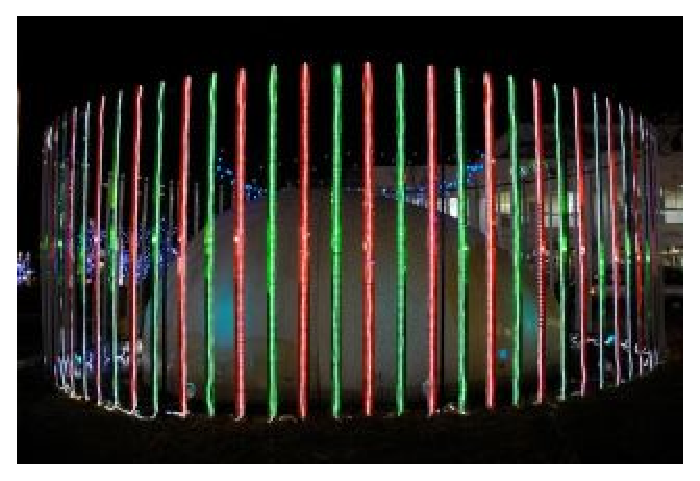
\includegraphics[width=\linewidth]{figs/egg_R.eps}
			\caption{右目用}
			\label{fig:egg_R}
		\end{minipage}
		\hspace{0.01\linewidth}
		\begin{minipage}[t]{0.49\linewidth}
			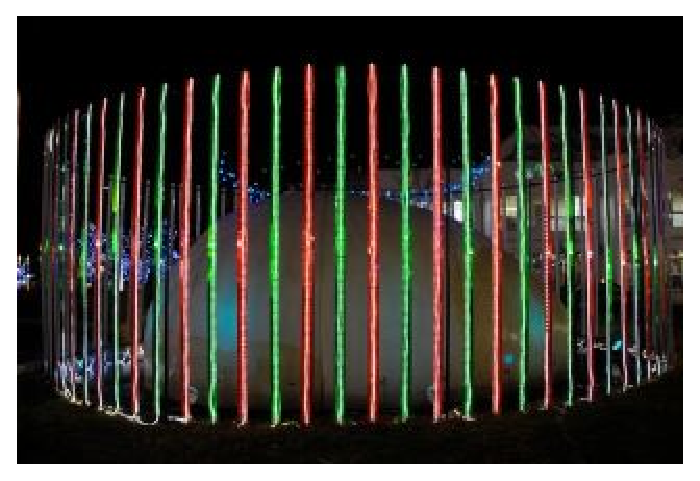
\includegraphics[width=\linewidth]{figs/egg_L.eps}
			\caption{左目用}
			\label{fig:egg_L}
		\end{minipage}
         \end{figure}
	実はこの象の卵の像の中に本当の卵が隠されている可能性もあるため、
	最新の技術を用いて非破壊的に内部を調査する。

	象の卵の研究の計画と方法は...
%end  研究計画 ====================
}

